\documentclass[aspectratio=169]{beamer}
\setbeamertemplate{navigation symbols}{}
\usepackage{color,amsmath,comment, subfigure}
\usepackage{booktabs}
\def\vf{\vfill}
\usepackage{url}

\def\imagetop#1{\vtop{\null\hbox{#1}}} %http://tex.stackexchange.com/questions/23521/tabular-vertical-alignment-to-top

%\setbeameroption{show notes}

%%%%%%%%%%%%%%%%%%%%%%%%%%
\title[]{Class 18: Social media and individuals}
\author[]{Matthew J. Salganik}
\institute[]{Sociology 204: Social Networks\\Princeton University}
\date[]{
2/3 The Facebook deprivation experiment
\vfill

\begin{flushleft}
\vspace{0.6in}

\includegraphics[width=0.1\textwidth]{figures/cc.png}
\end{flushleft}
}

\begin{document}
%%%%%%%%%%%%%%%%%%%%%%%%%%%
\frame{\titlepage}
%%%%%%%%%%%%%%%%%%%%%%%%%%%
\begin{frame}

\begin{center}

\includegraphics[width=0.4\textwidth]{figures/fb_logo}
\end{center}

Facebook has 1.84 billion \emph{daily} active users.  What is the effect of Facebook on its users?

\tiny{\url{https://investor.fb.com/investor-news/press-release-details/2021/Facebook-Reports-Fourth-Quarter-and-Full-Year-2020-Results/default.aspx}}
\end{frame}
%%%%%%%%%%%%%%%%%%%%%%
\begin{frame}

\begin{itemize}
\item We could compare Facebook users to non-Facebook users, but there might be lots of other differences. \pause
\item Among Facebook users, we could compare ``light'' users to ``heavy'' users, but again there might be lots of other differences. 
\end{itemize}

\end{frame}
%%%%%%%%%%%%%%%%%%%%%%
\begin{frame}

Allcott et al.\ run an randomized control trial (an ``experiment'').

\end{frame}
%%%%%%%%%%%%%%%%%%%%%%
\begin{frame}

\begin{center}

\includegraphics[width=0.6\textwidth]{figures/allcott_welfare_2020_figa1}
\end{center}

\end{frame}
%%%%%%%%%%%%%%%%%%%%%
\begin{frame}

\begin{center}
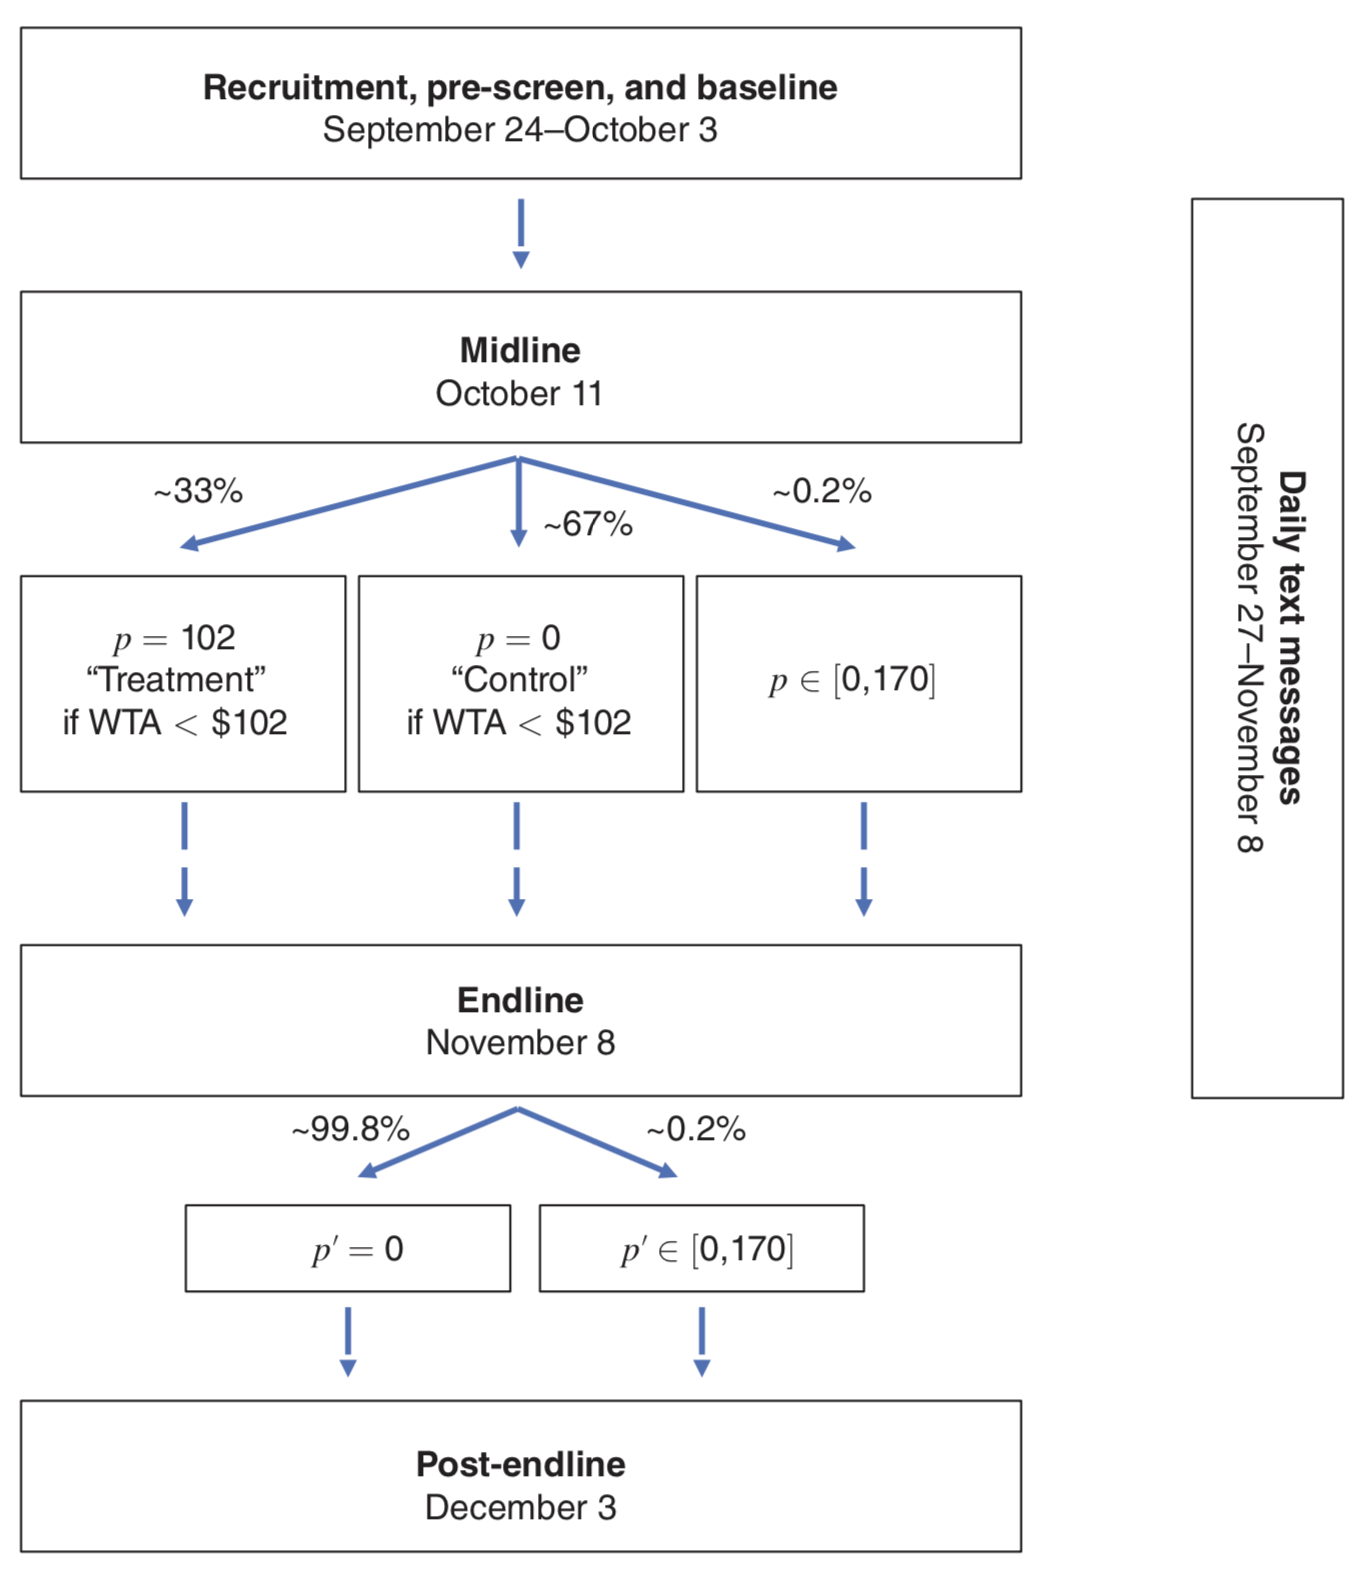
\includegraphics[width=0.5\textwidth]{figures/allcott_welfare_2020_fig1}
\end{center}

This design means that the collection of people in the treatment group are the same as people in the control group.

\note{
People were paid \$102 to deactivate. 
}

\end{frame}
%%%%%%%%%%%%%%%%%%%%%
\begin{frame}

Thinking about external validity: who is in the experiment? \pause

\begin{center}
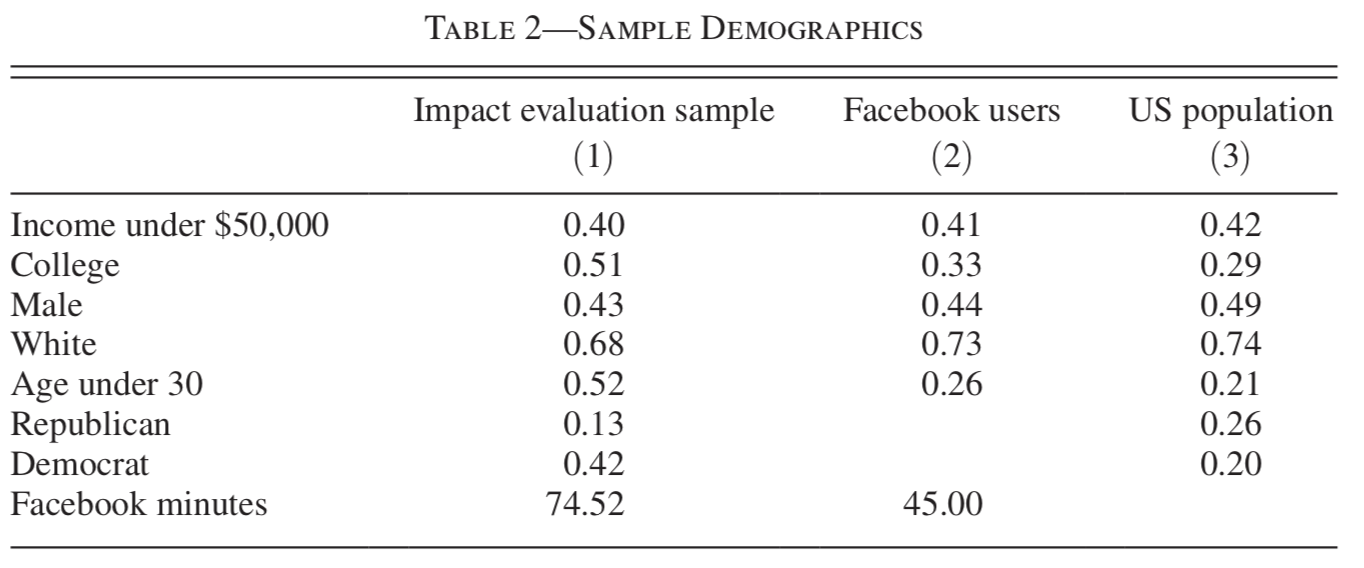
\includegraphics[width=0.8\textwidth]{figures/allcott_welfare_2020_tab2}
\end{center}

\begin{itemize}
\item impact evaluation sample is older, more educated, and uses Facebook more
\item note that this experiment might not include the youngest users who might be most harmed by Facebook
\end{itemize}

\end{frame}
%%%%%%%%%%%%%%%%%%%%%
\begin{frame}

Thinking about internal validity: was their differential compliance or attrition? \pause

\begin{center}
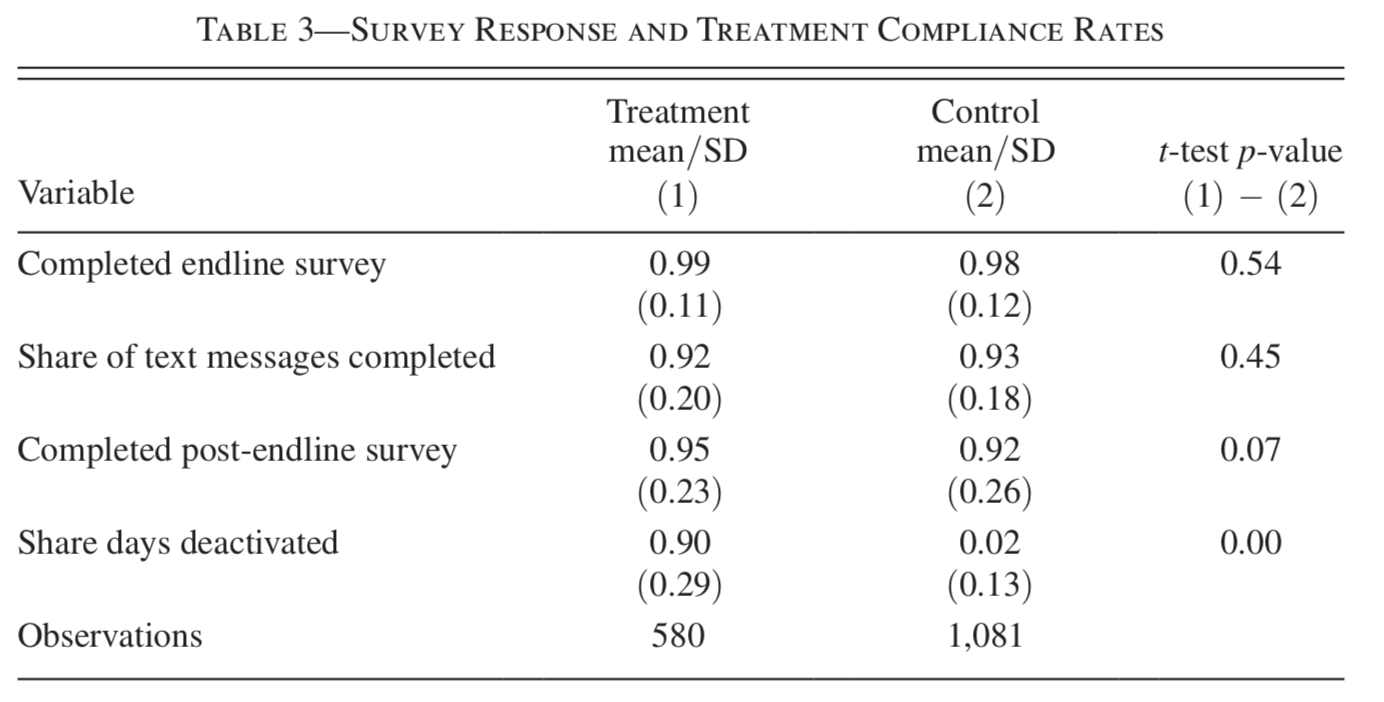
\includegraphics[width=0.8\textwidth]{figures/allcott_welfare_2020_tab3}
\end{center}

\begin{itemize}
\item compliance was high and there was little attrition 
\end{itemize}

\end{frame}
%%%%%%%%%%%%%%%%%%%%%
\begin{frame}

\begin{center}
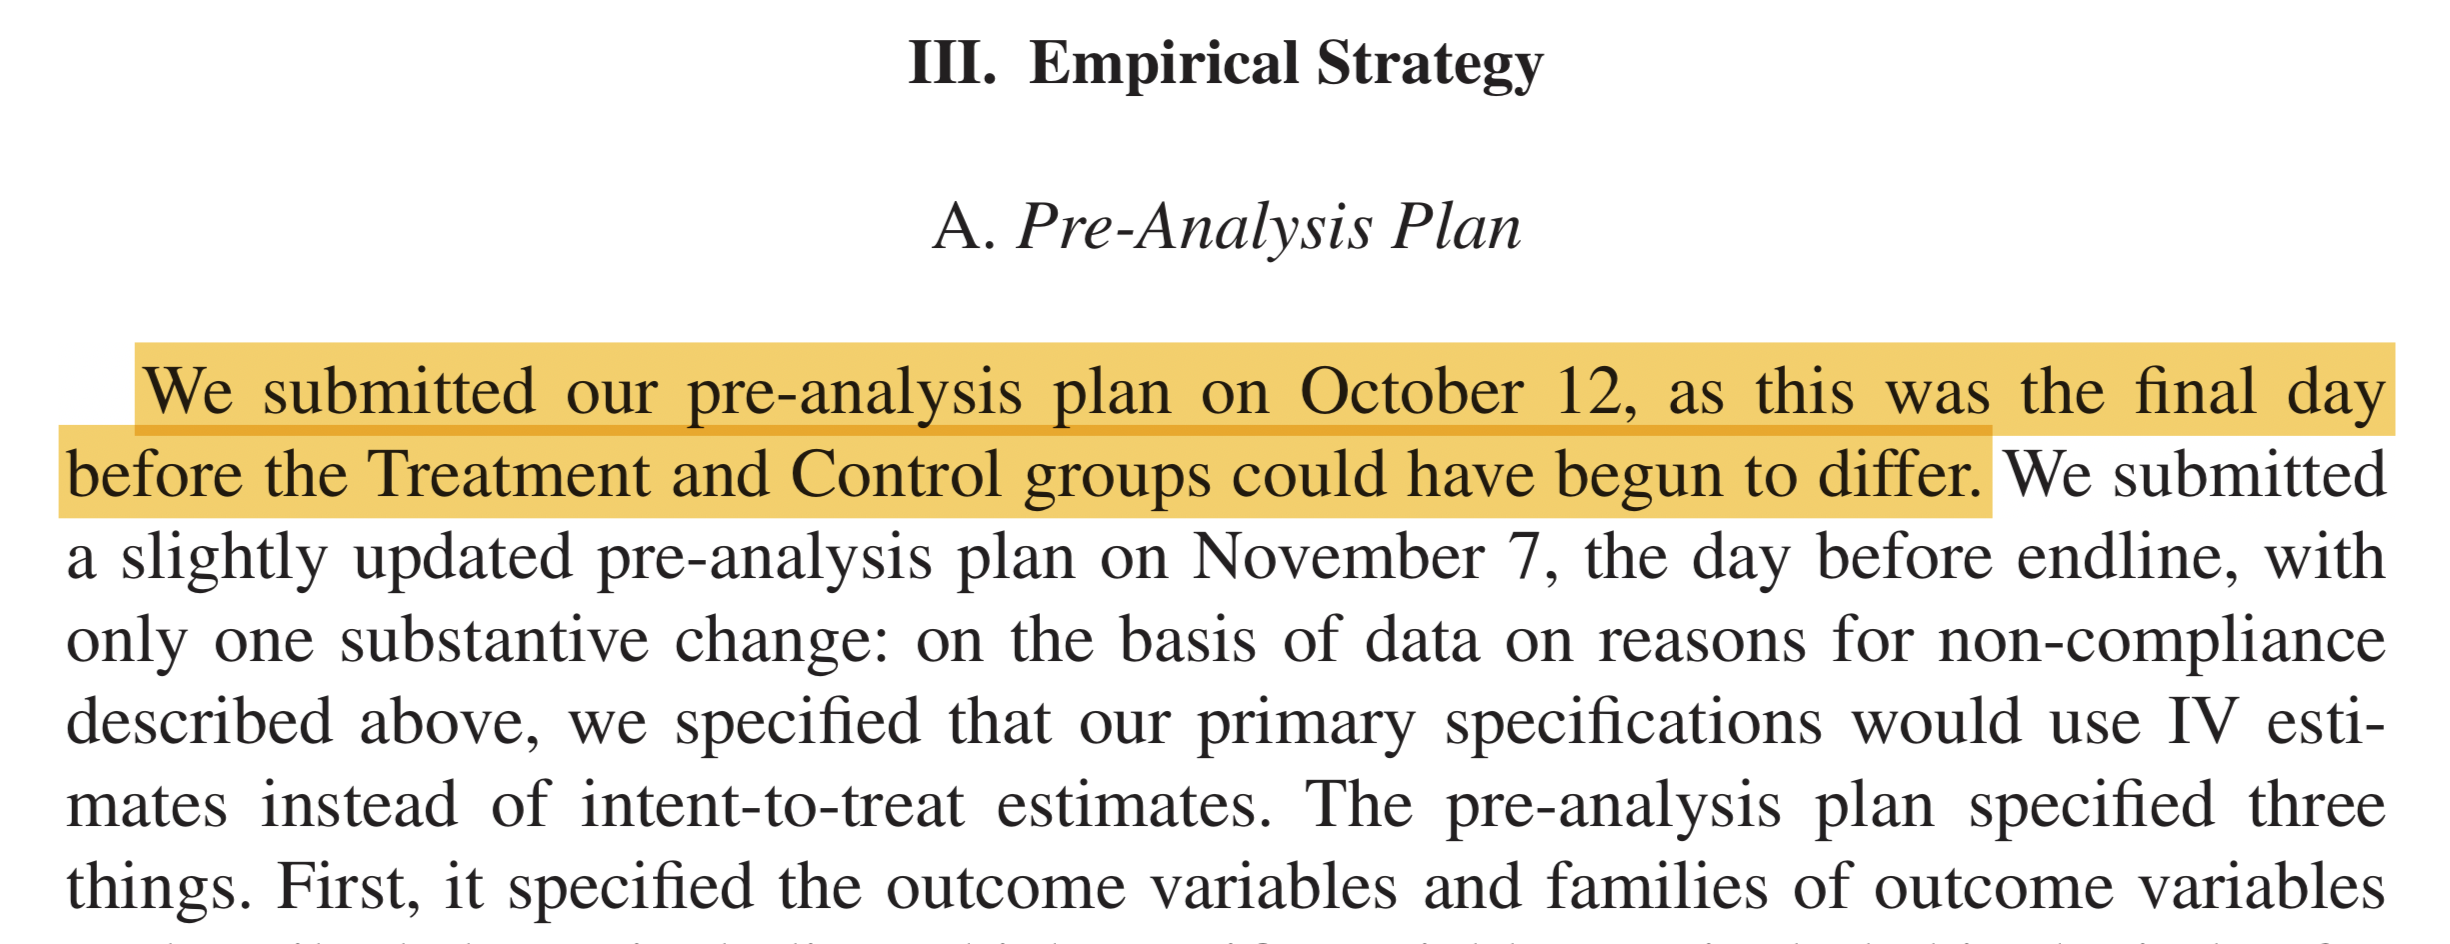
\includegraphics[width=1\textwidth]{figures/allcott_welfare_2020_preanalysis}
\end{center}

\end{frame}
%%%%%%%%%%%%%%%%%%%%%
\begin{frame}

Nine families of outcome variables, focus on politics (perhaps because experiment was right before an election)
\begin{itemize}
\item Substitute Time Uses
\item Social Interaction
\item Substitute News Sources
\item News Knowledge
\item Political Engagement
\item Political Polarization
\item Subjective Well-Being
\item Post-Experiment Facebook Use
\item Opinions about Facebook
\end{itemize}

\end{frame}
%%%%%%%%%%%%%%%%%%%%%
\begin{frame}

\begin{itemize}
\item Endpoint
\begin{itemize}
\item Substitution
\item Well-being
\item News and politics
\end{itemize}
\item Post-deactivation
\end{itemize}

\end{frame}
%%%%%%%%%%%%%%%%%%%%%
\begin{frame}

\begin{itemize}
\item Endpoint
\begin{itemize}
\item \textcolor{blue}{Substitution}
\item Well-being
\item News and politics
\end{itemize}
\item Post-deactivation
\end{itemize}

\end{frame}
%%%%%%%%%%%%%%%%%%%%%
\begin{frame}

\begin{center}
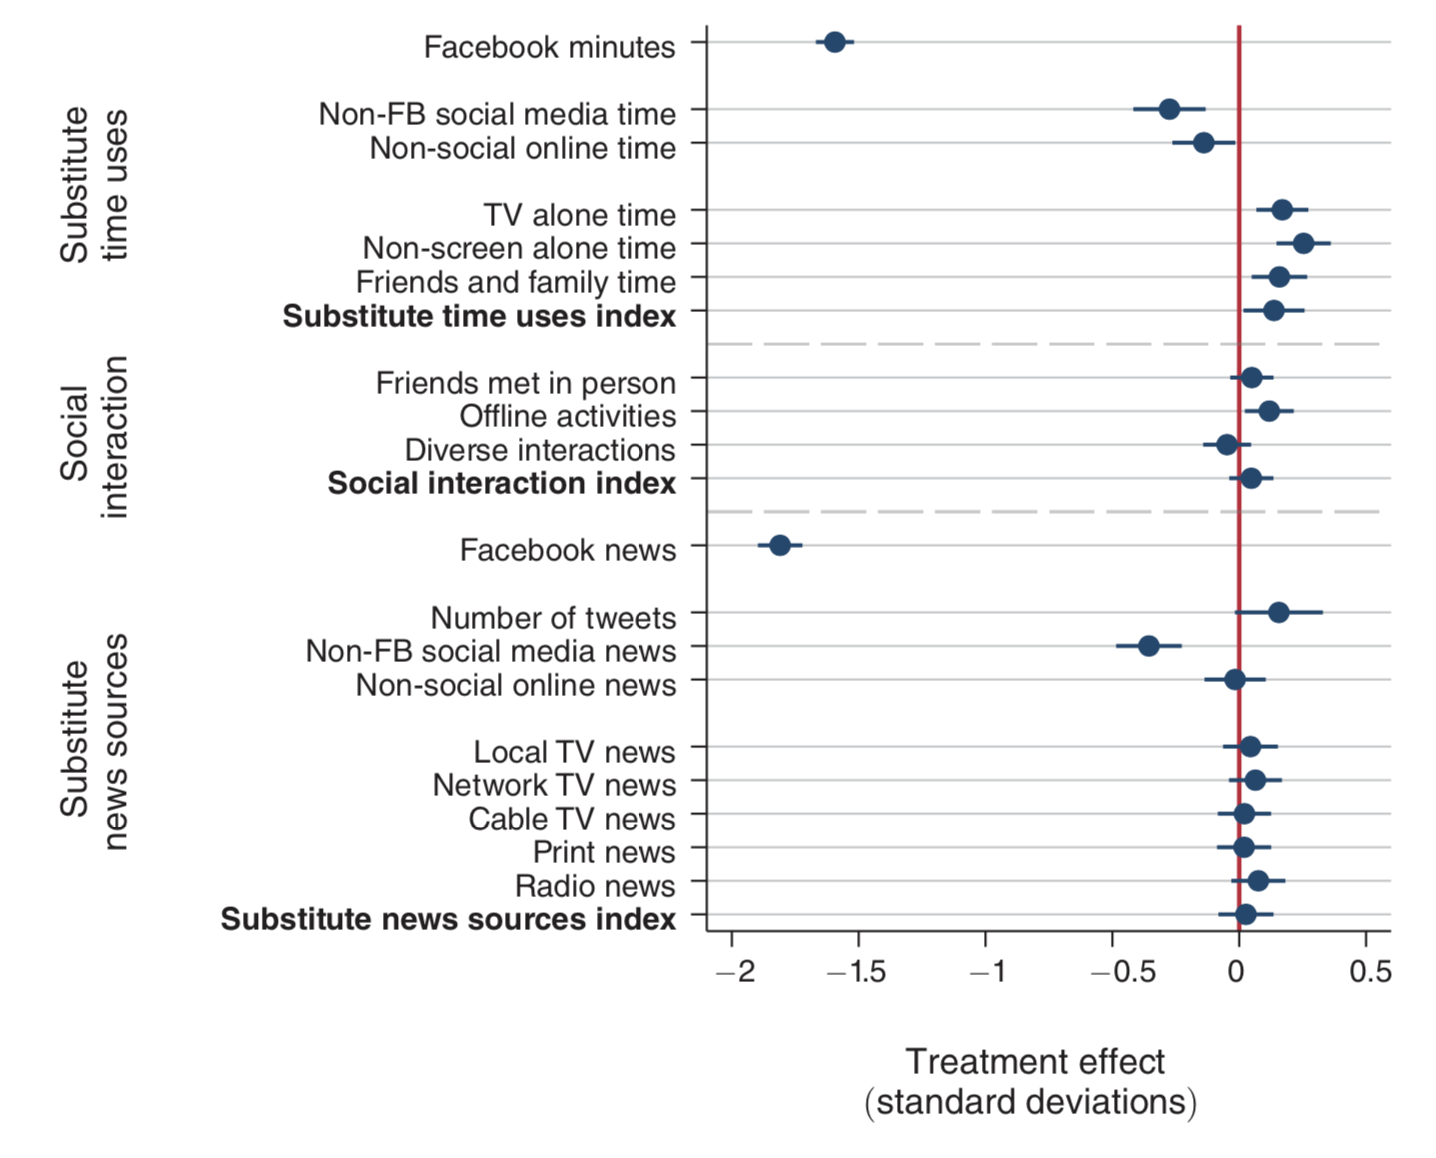
\includegraphics[width=0.5\textwidth]{figures/allcott_welfare_2020_fig2}
\end{center}

\begin{itemize}
\item reduced time on FB \pause
\item slightly reduced time on other social media \pause
\item slightly more time with offline activities \pause
\item didn't impact non-social media source of news \pause
\end{itemize}
\vfill
All of these are measured in terms of standard deviation units in the control group

\end{frame}
%%%%%%%%%%%%%%%%%%%%%
\begin{frame}

\begin{itemize}
\item Endpoint
\begin{itemize}
\item Substitution
\item \textcolor{blue}{Well-being}
\item News and politics
\end{itemize}
\item Post-deactivation
\end{itemize}

\end{frame}
%%%%%%%%%%%%%%%%%%%%%
\begin{frame}

\begin{center}
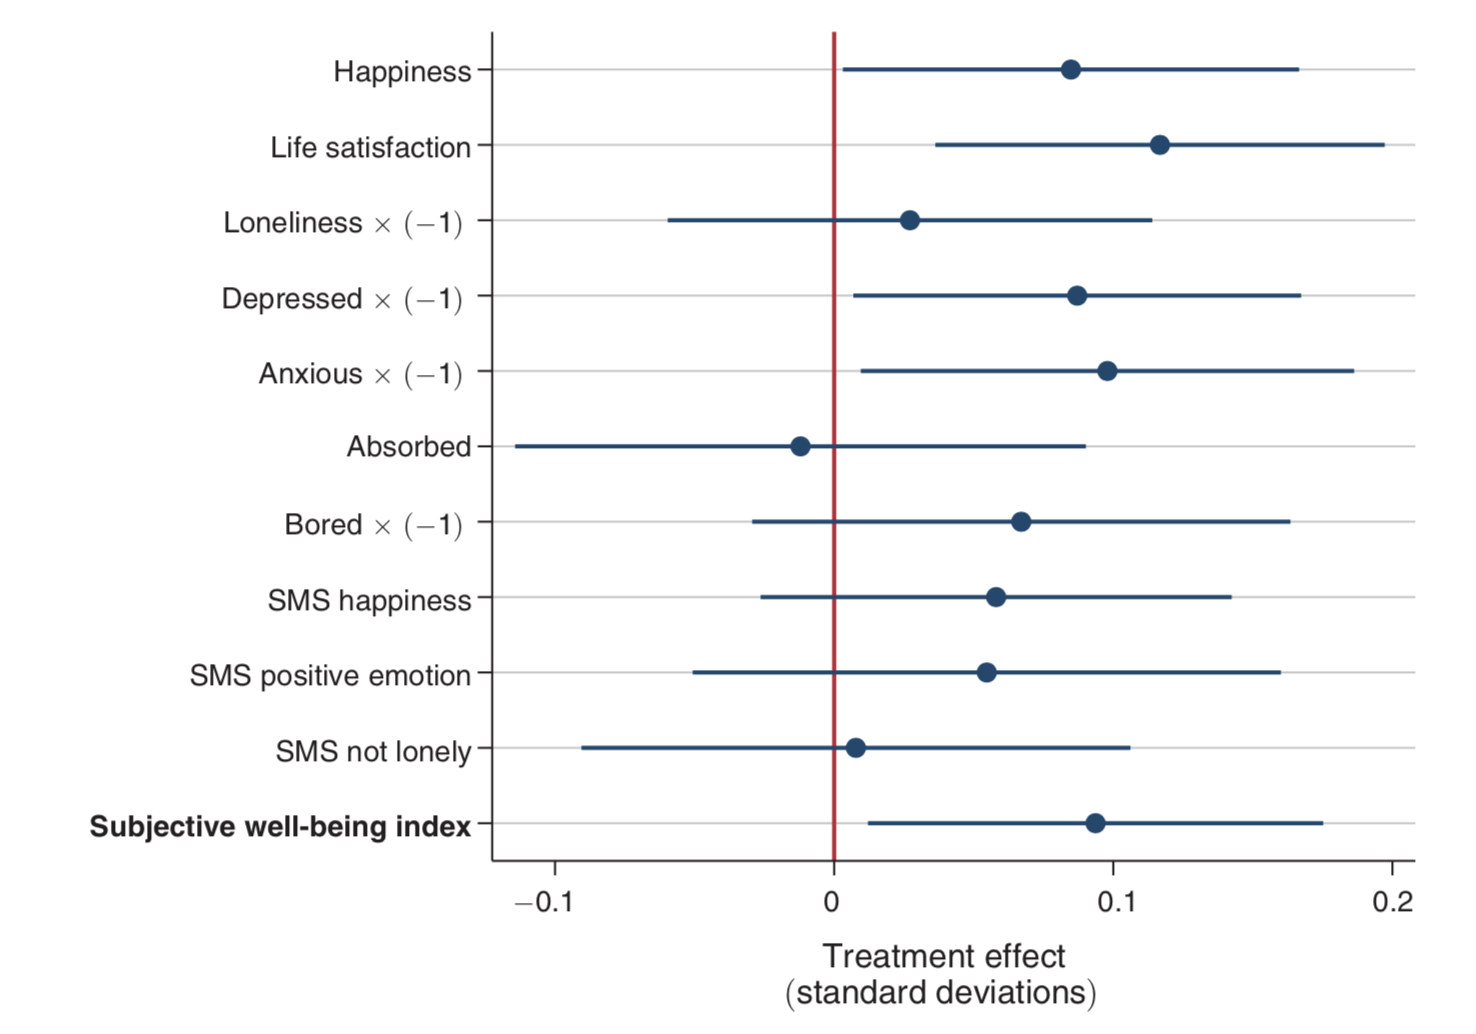
\includegraphics[width=0.7\textwidth]{figures/allcott_welfare_2020_fig5}
\end{center}

\begin{itemize}
\item ``small'' improvements in most measures
\end{itemize}

\end{frame}
%%%%%%%%%%%%%%%%%%%%%
\begin{frame}

\begin{center}
\only<1>{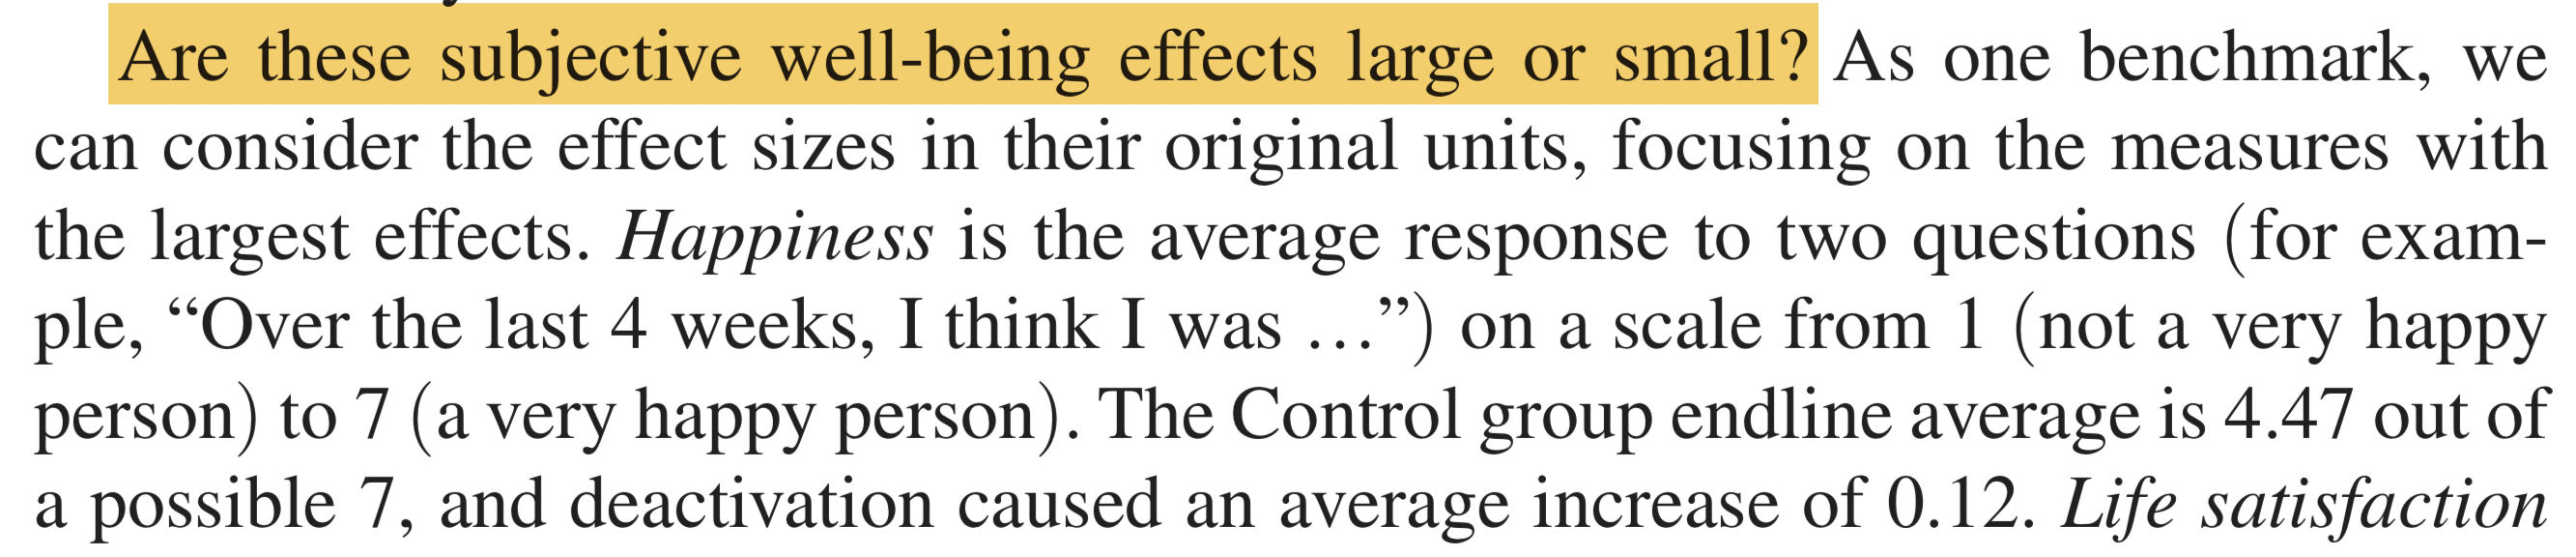
\includegraphics[width=0.9\textwidth]{figures/allcott_welfare_2020_swb_size1}}%
\only<2>{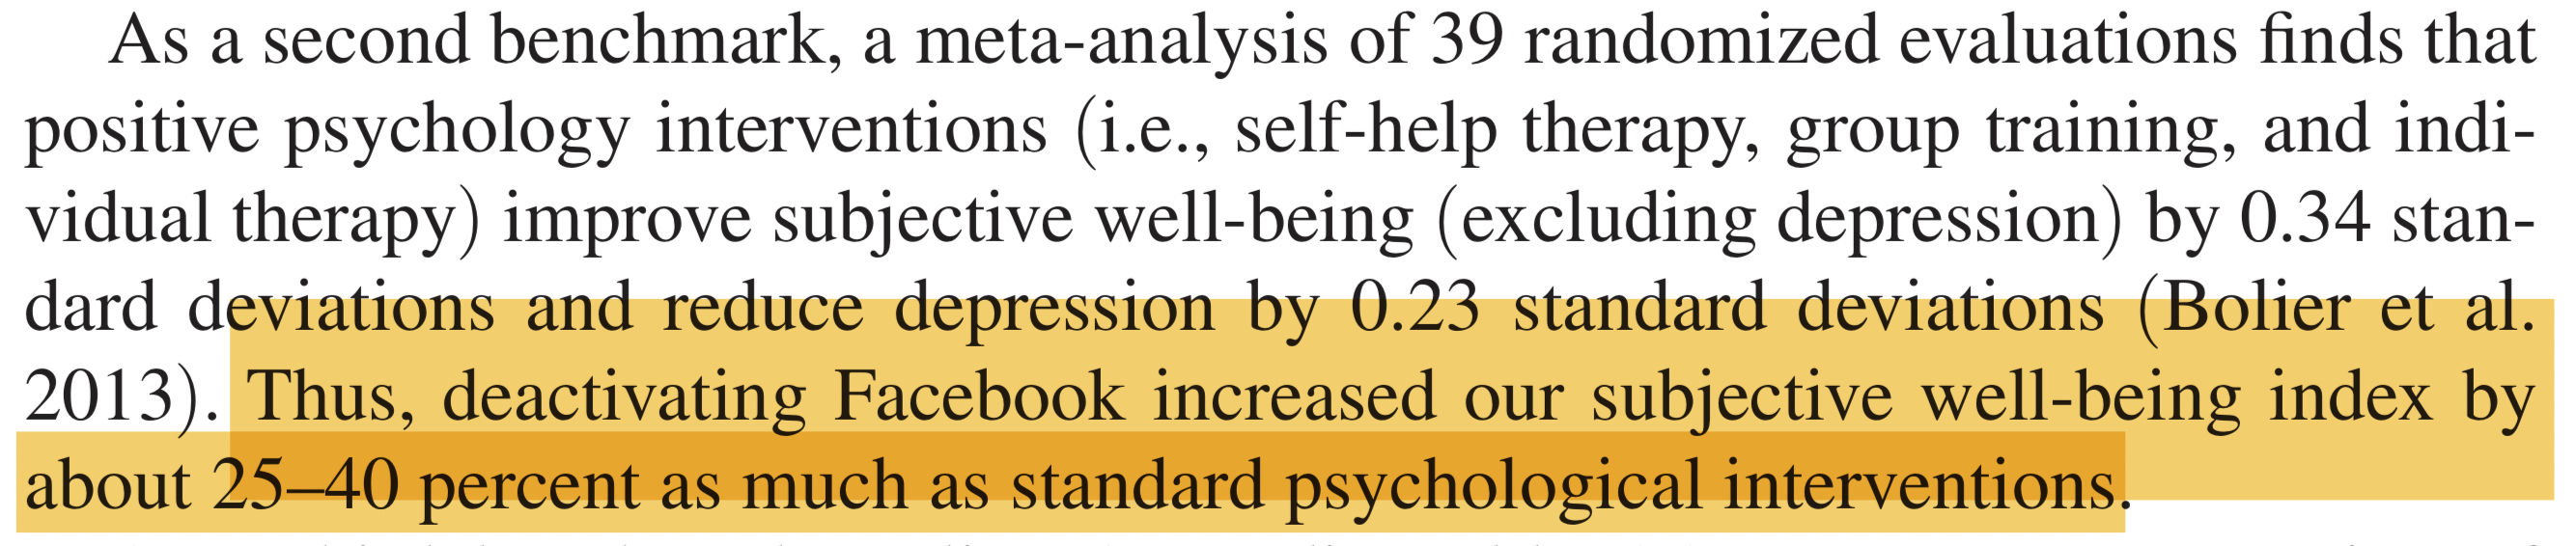
\includegraphics[width=0.9\textwidth]{figures/allcott_welfare_2020_swb_size2}}%
\only<3>{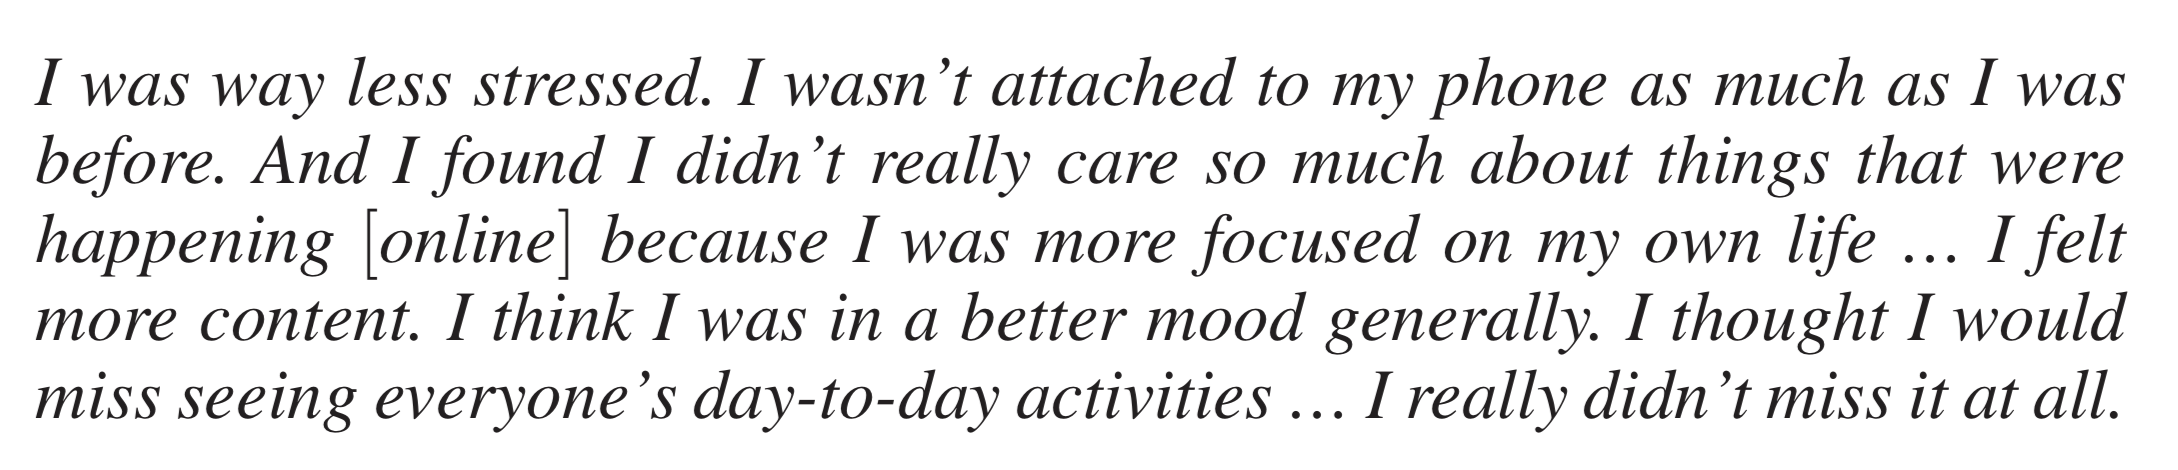
\includegraphics[width=0.9\textwidth]{figures/allcott_welfare_2020_swb_quote}}%
\end{center}

\note{
Note how they mix quantitative and qualitative evidence
}

\end{frame}
%%%%%%%%%%%%%%%%%%%%%
\begin{frame}

\begin{itemize}
\item Endpoint
\begin{itemize}
\item Substitution
\item Well-being
\item \textcolor{blue}{News and politics}
\end{itemize}
\item Post-deactivation
\end{itemize}

\end{frame}
%%%%%%%%%%%%%%%%%%%%%
\begin{frame}

\begin{center}
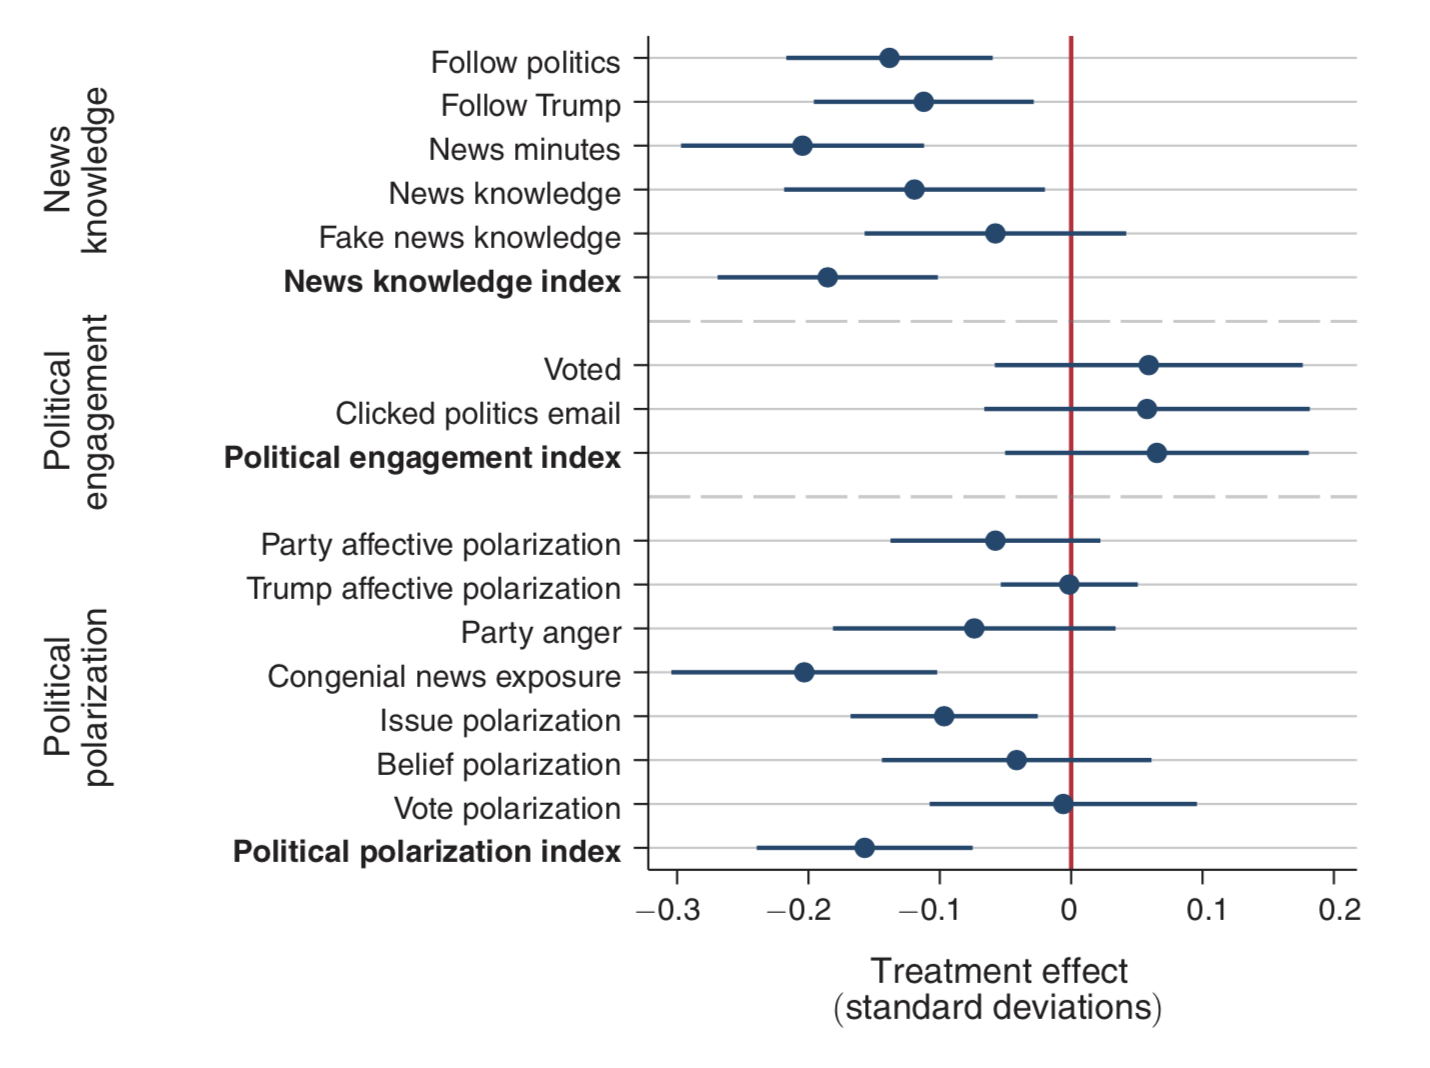
\includegraphics[width=0.6\textwidth]{figures/allcott_welfare_2020_fig3}
\end{center}

\begin{itemize}
\item less news knowledge \pause
\item less political polarization
\end{itemize}

\end{frame}
%%%%%%%%%%%%%%%%%%%%%
\begin{frame}

\begin{center}
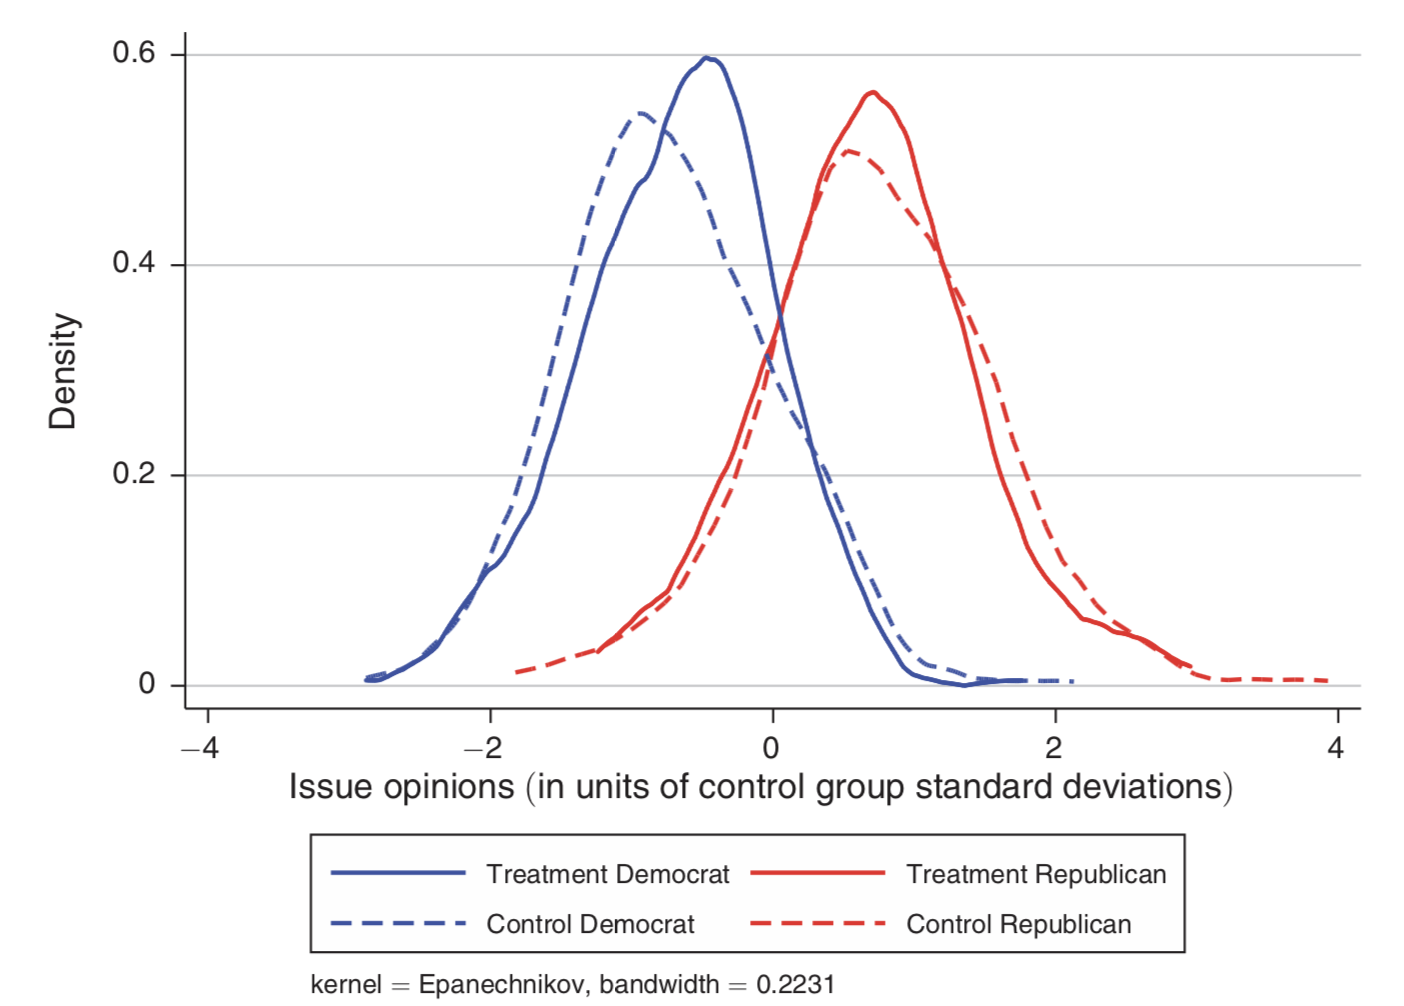
\includegraphics[width=0.8\textwidth]{figures/allcott_welfare_2020_fig4}
\end{center}

\end{frame}
%%%%%%%%%%%%%%%%%%%%%
\begin{frame}

Heterogenous treatment effects: are the treatment effects the same for everyone? \pause

\begin{center}
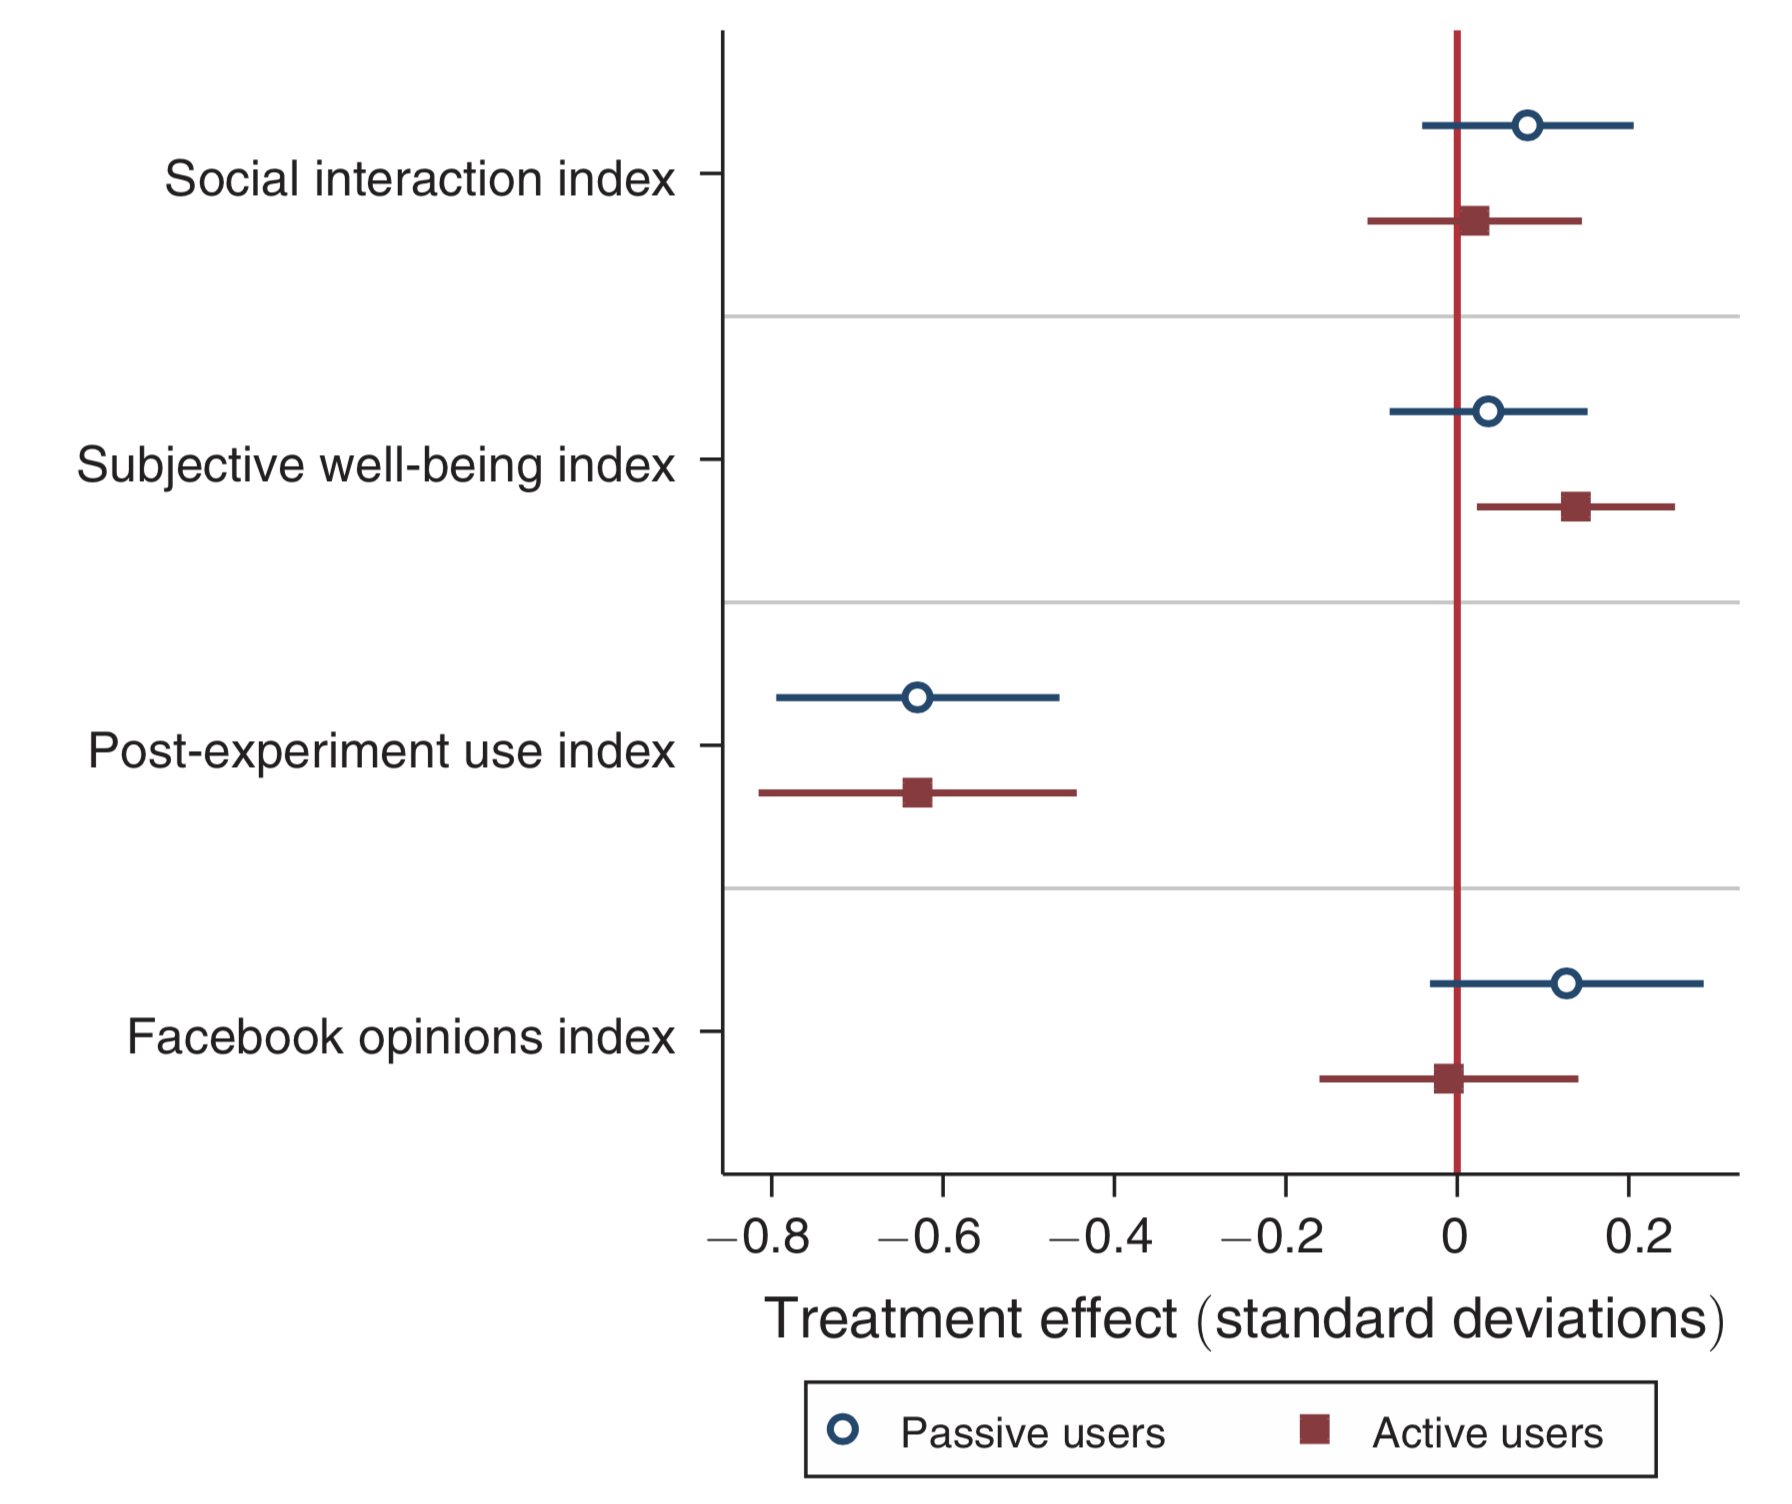
\includegraphics[width=0.5\textwidth]{figures/allcott_welfare_2020_fig9top}
\end{center}

\begin{itemize}
\item Effects are similar for active and passive users
\end{itemize}

\vfill 
Can't learn about heterogeneity from self-experimentation

\end{frame}
%%%%%%%%%%%%%%%%%%%%%
\begin{frame}

\begin{center}
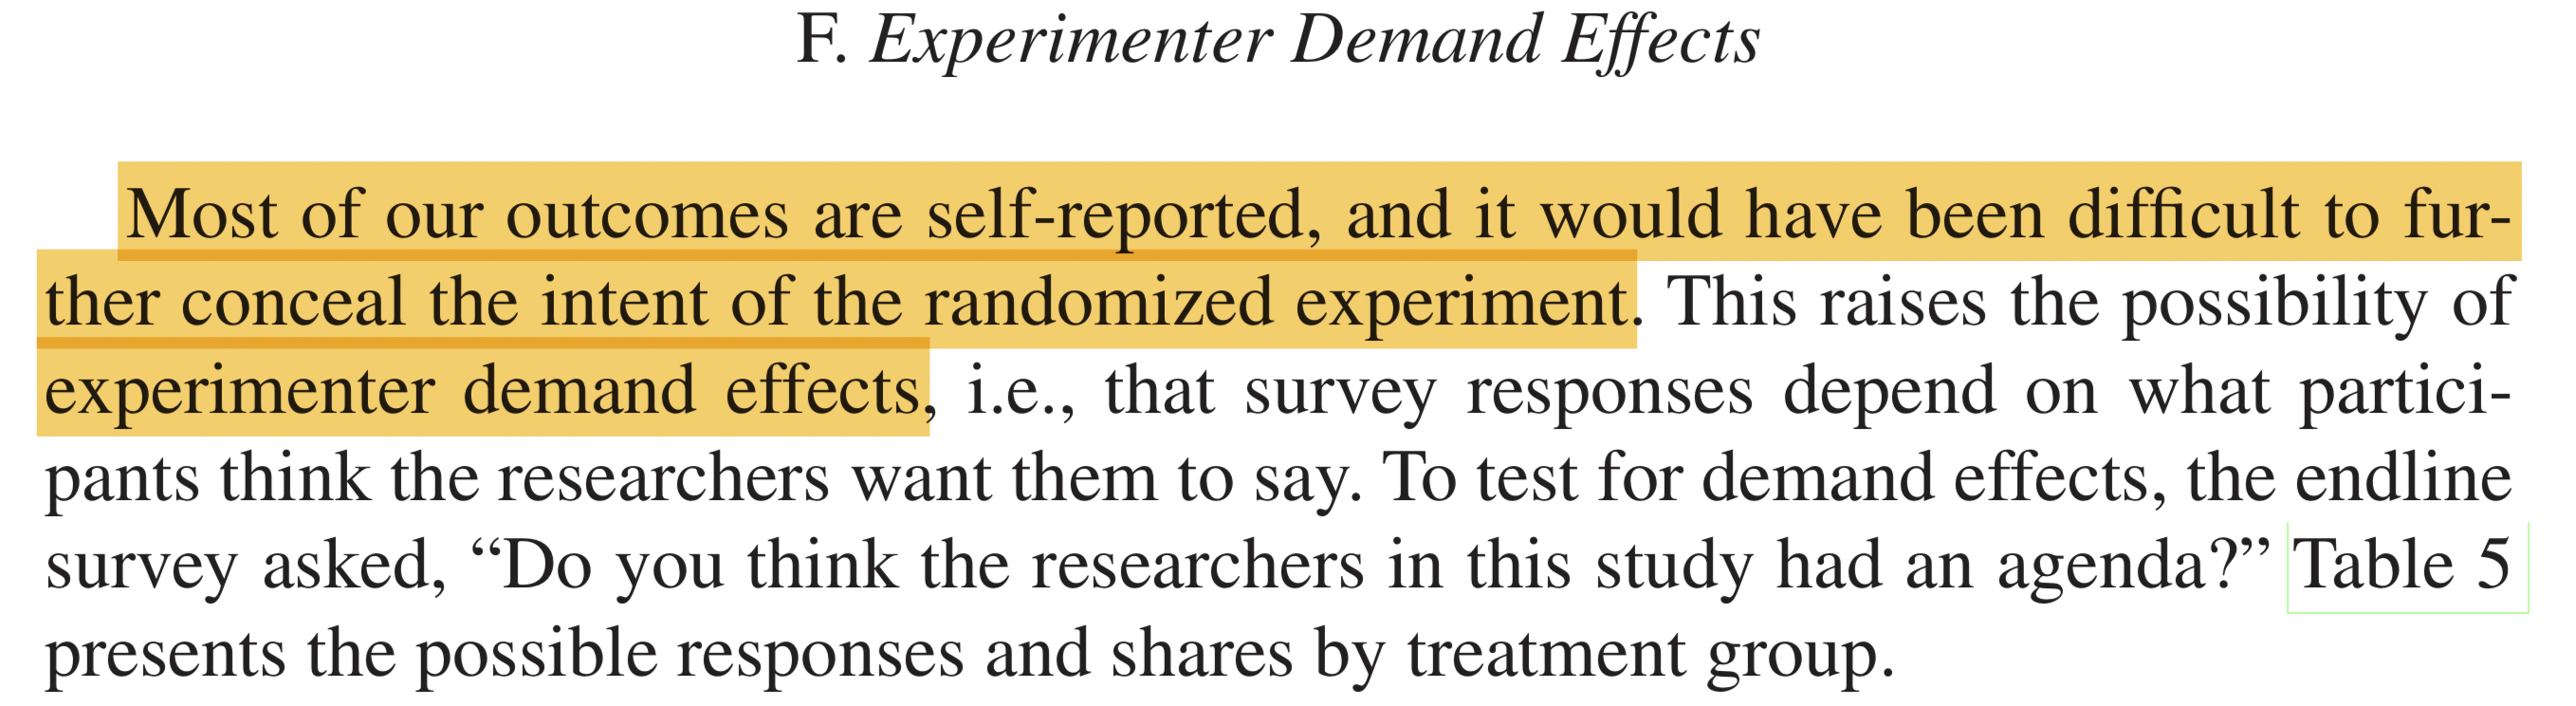
\includegraphics[width=0.8\textwidth]{figures/allcott_welfare_2020_demandeffects}
\end{center}

\pause
\begin{itemize}
\item double-blind experiments \pause
\item single-blind experiments \pause
\item unblinded experiments \pause
\item self experiments
\end{itemize}

\end{frame}
%%%%%%%%%%%%%%%%%%%%%
\begin{frame}

\begin{itemize}
\item Endpoint
\begin{itemize}
\item Substitution
\item Well-being
\item News and politics
\end{itemize}
\item \textcolor{blue}{Post-deactivation}
\end{itemize}

\end{frame}
%%%%%%%%%%%%%%%%%%%%%
\begin{frame}

\begin{center}
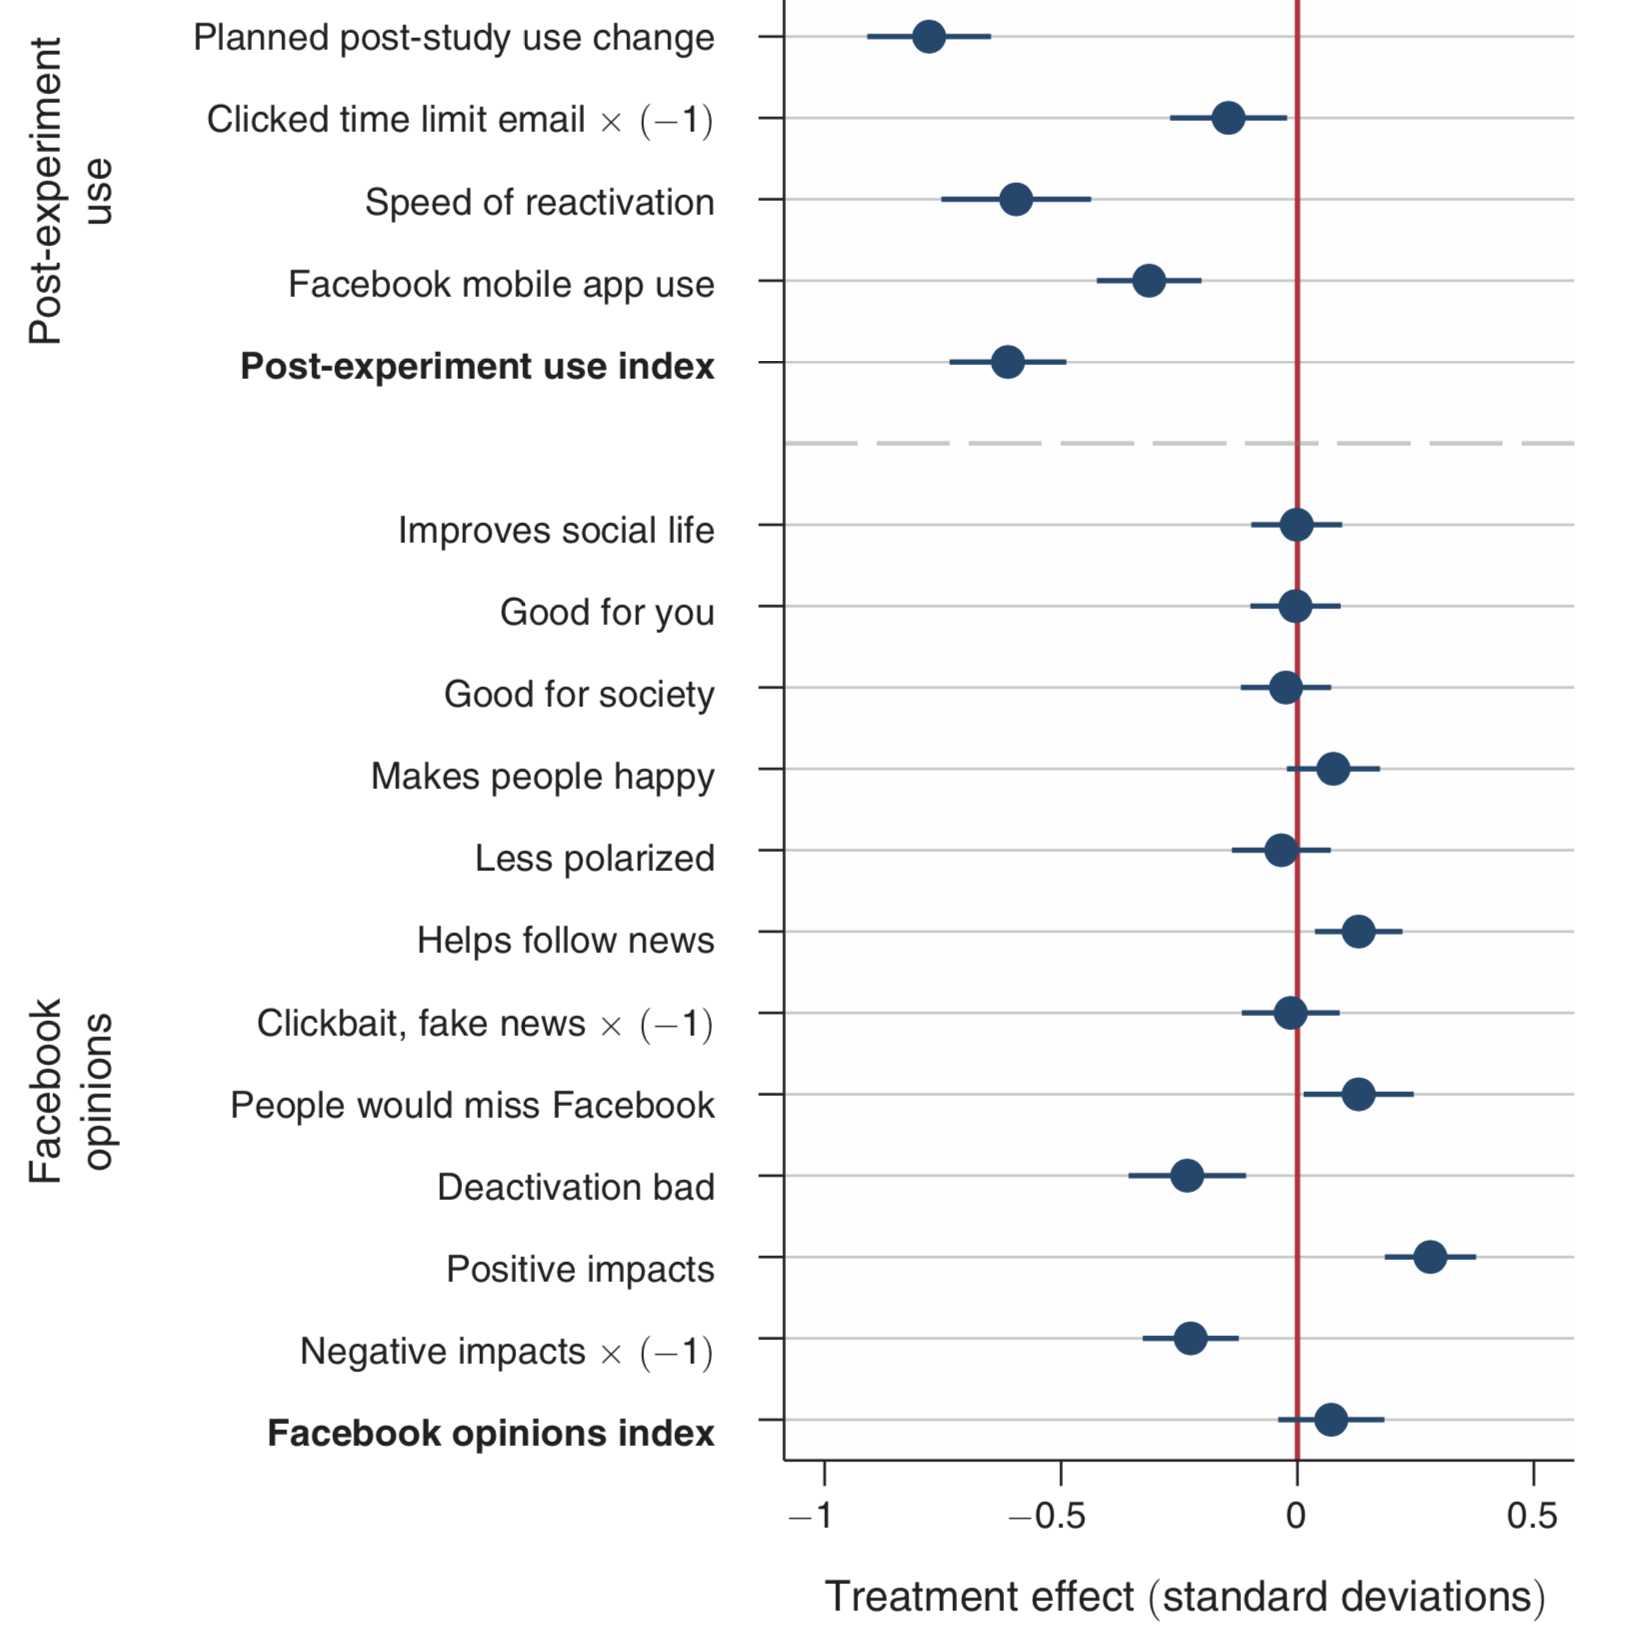
\includegraphics[width=0.5\textwidth]{figures/allcott_welfare_2020_fig6}
\end{center}

\begin{itemize}
\item wanting to use FB less in the future (about 20\% reduction in time used)
\item more awareness of the good and bad aspects of FB
\end{itemize}

\end{frame}
%%%%%%%%%%%%%%%%%%%
\begin{frame}

\begin{center}
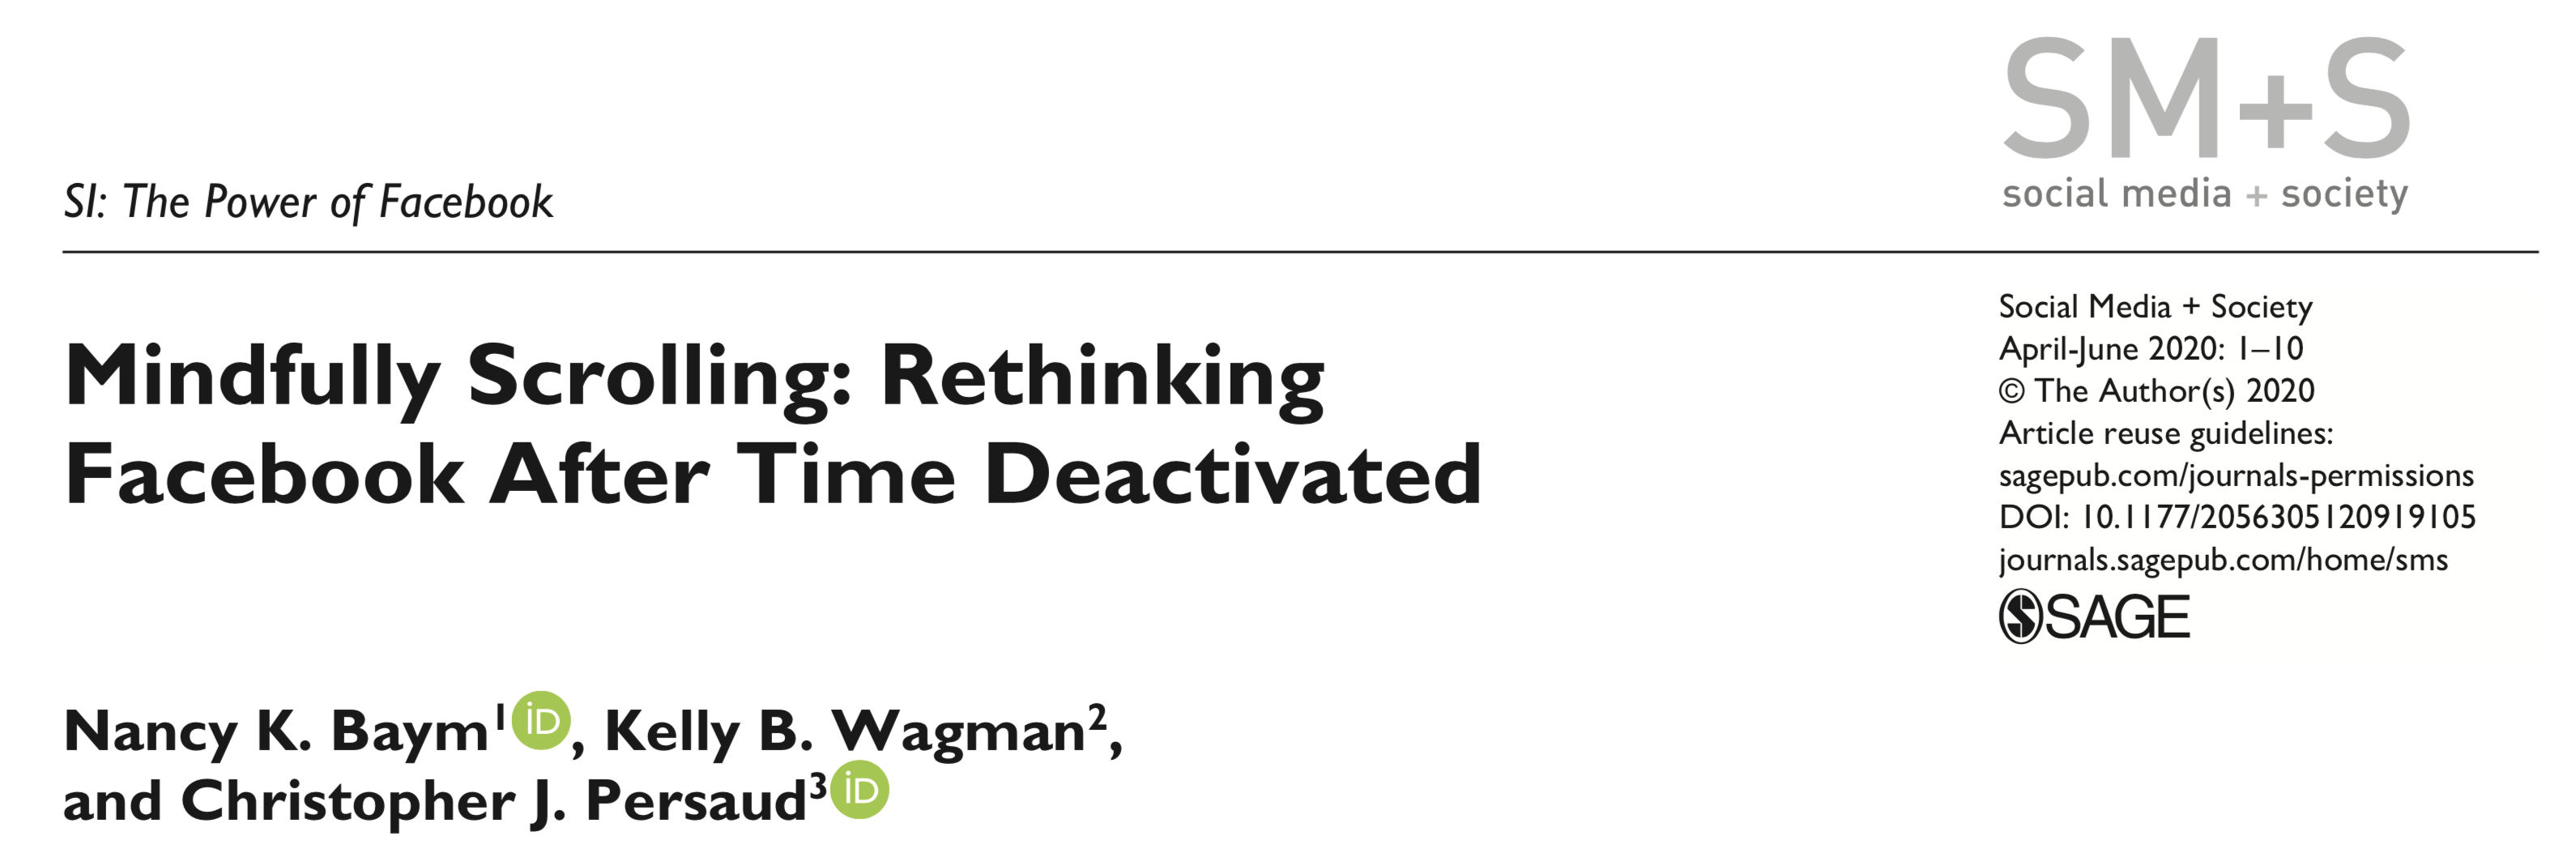
\includegraphics[width=0.8\textwidth]{figures/baym_mindfully_2020_title}
\end{center}

\note{
qualitative reading of responses
}

\end{frame}
%%%%%%%%%%%%%%%%%%%
\begin{frame}

Baym et al.\ describe changes in two areas:
\begin{itemize}
\item Awareness: \only<2->{Automaticity, FB's value}
\item Behavior: \only<3>{Tweaking settings to avoid certain things, not structural reform}
\end{itemize}

\end{frame}
%%%%%%%%%%%%%%%%%%%
\begin{frame}

\begin{center}
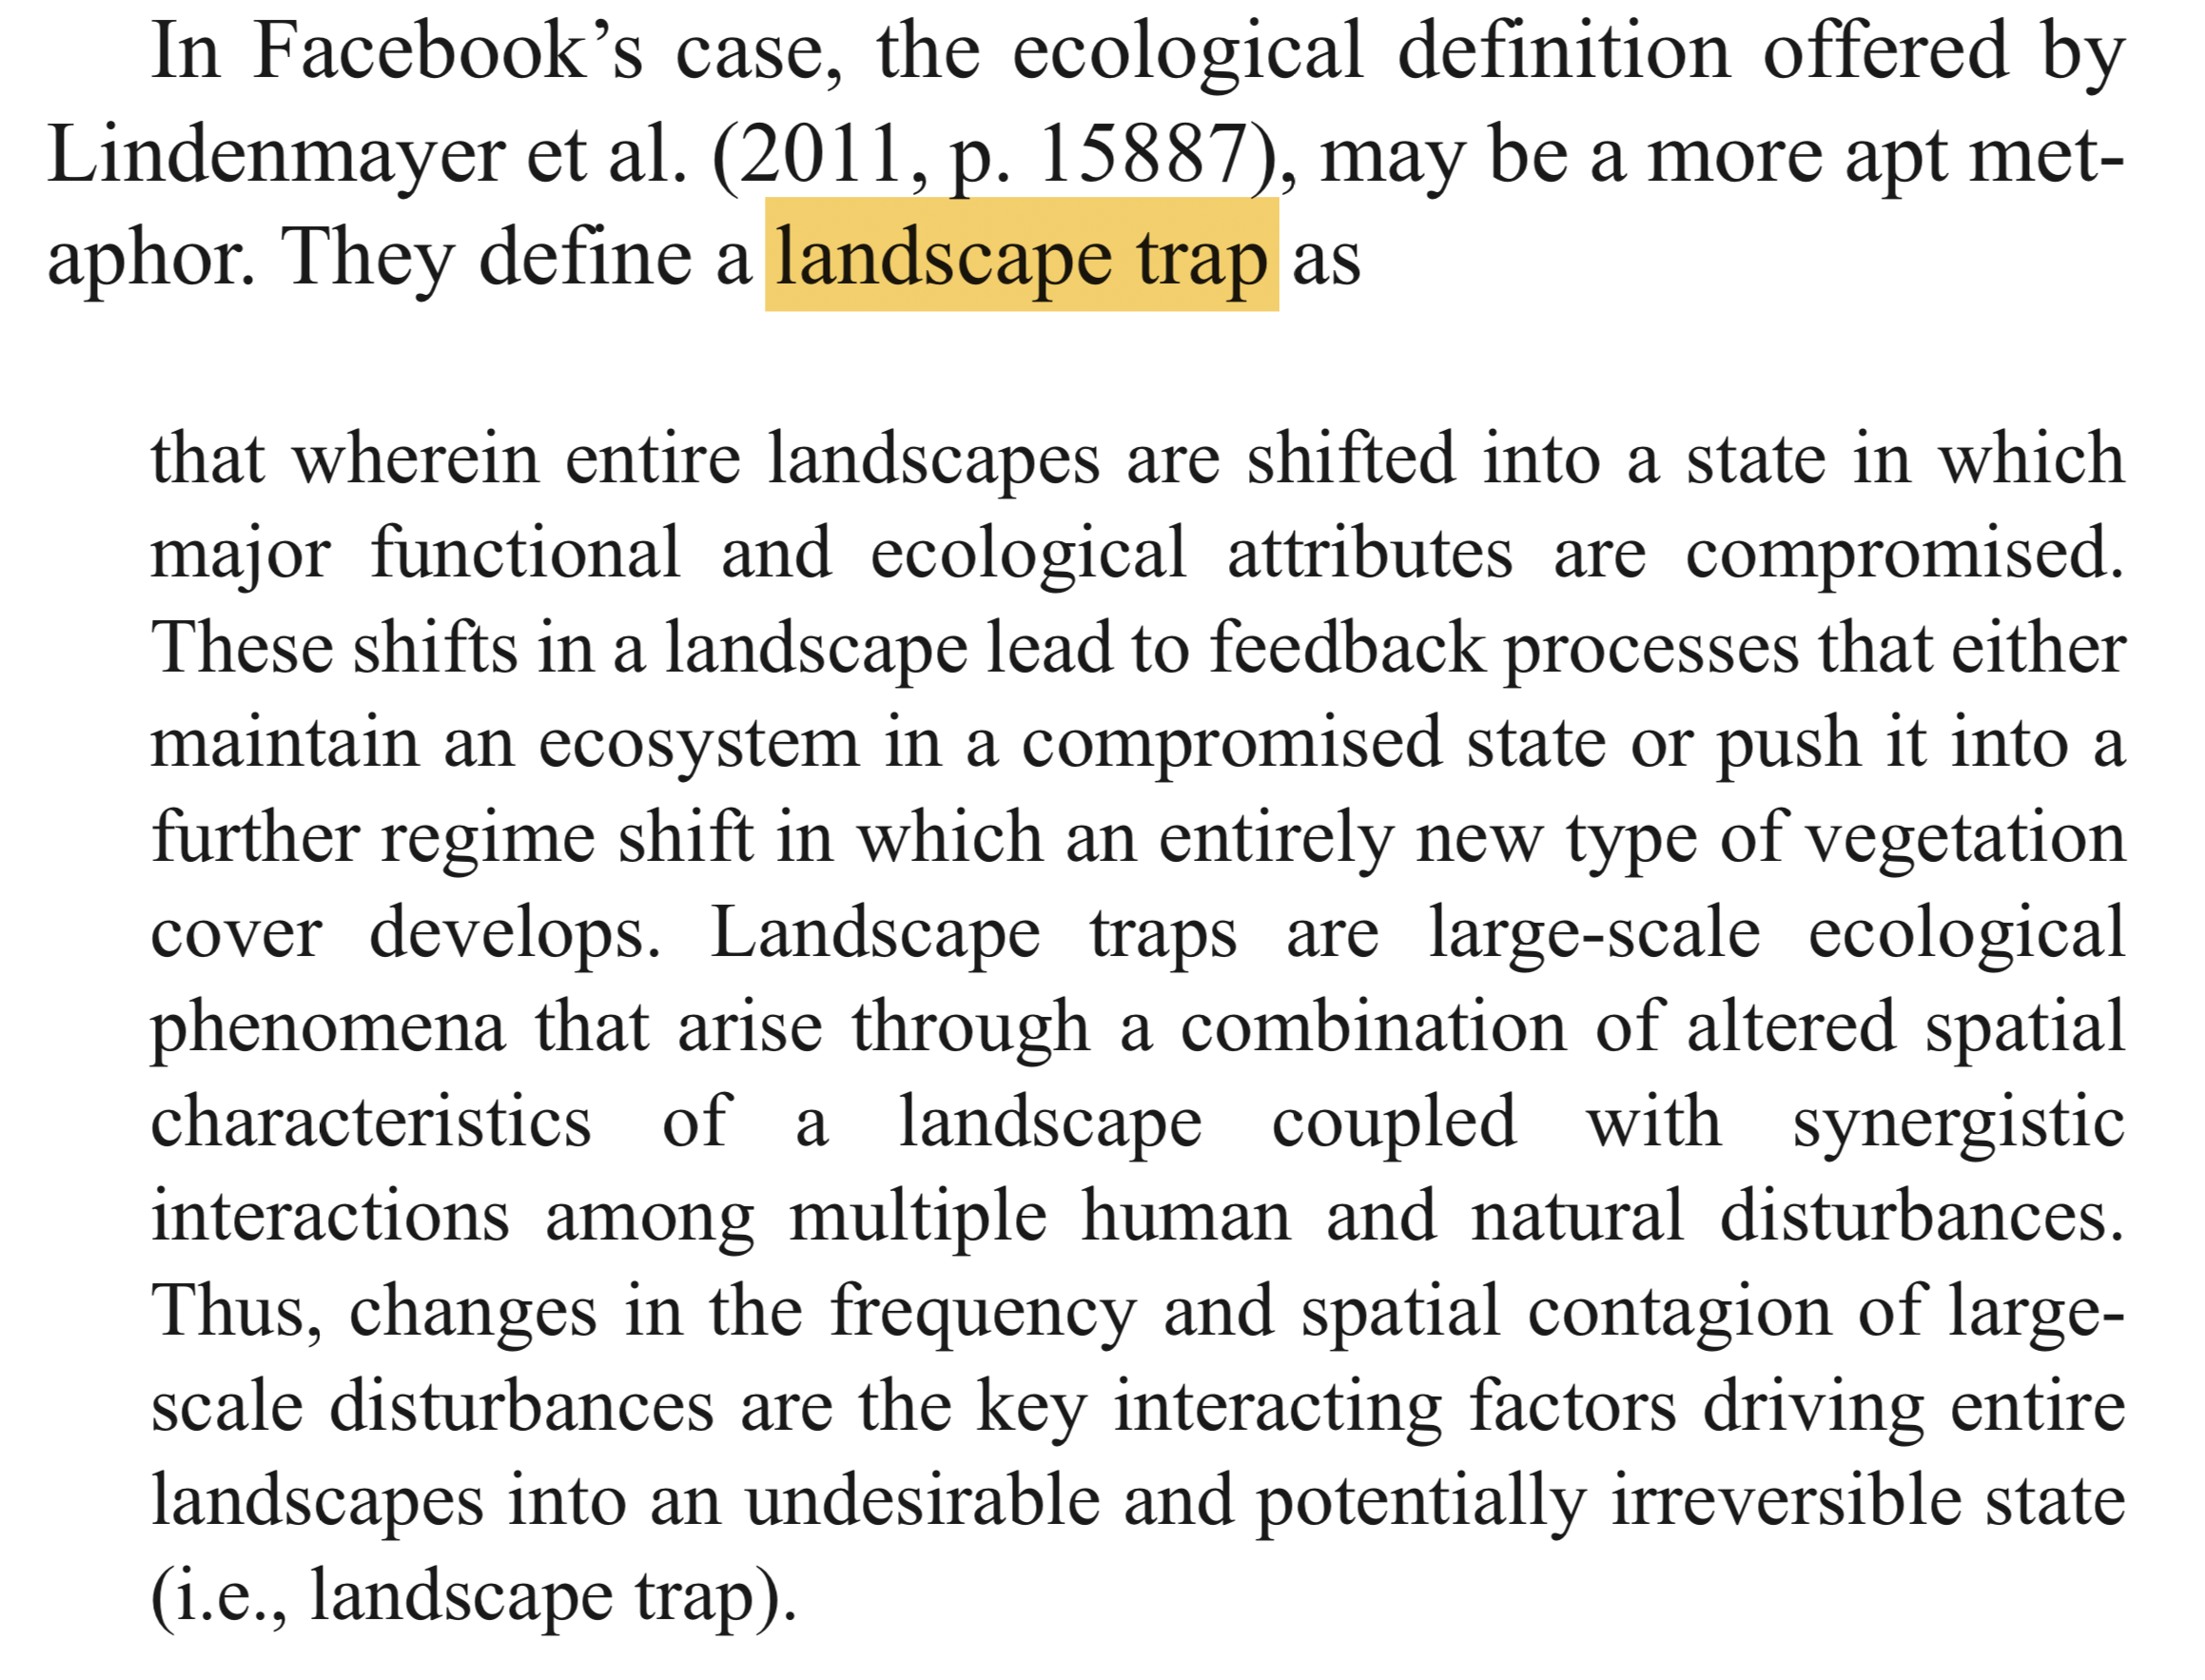
\includegraphics[width=0.6\textwidth]{figures/baym_mindfully_2020_landscape_trap}
\end{center}

\vfill 
\begin{itemize}
\item The landscape has shifted because of both intentional and unintentional action \pause
\item There is an important difference between one person deactivating FB and everyone deactivating FB
\end{itemize}

\note{
We will return to individual and structural changes next week
}

\end{frame}
%%%%%%%%%%%%%%%%%%%
\begin{frame}

Stepping back:
\begin{itemize}
\item Measuring and understanding the effect of social media on individuals is hard, in part because jingle-jangle problem and heterogeneity of social media and people \pause
\item Allcott et al.\ do a randomized controlled trial to measure the effect of FB on a sample of American users \pause
\item Being off FB for one month leads to 1) reduced online activity and increased offline activity 2) reduced factual news knowledge and political polarization 3) increased subjective well-being and 4) caused a large persistent reduction in post-experiment Facebook use \pause
\item Being off FB for one month also leads to new awareness about the good and bad aspects of FB 
\end{itemize}

\end{frame}
%%%%%%%%%%%%%%%%%%%
\begin{frame}

Now it is your turn: self-experimentation and social media

\end{frame}


\end{document}
